\subsection{平常時のグループ化の通信}
平常時のグループの通信フロー\ref{fig:default_data_flow}を述べる.グループ内の通信は,BLEを用いて,GLノードとGWノードの通信はLoRaWANを用いる.グループ内の通信は,インターバルが設けられ同期的に通信を行う.センサデータ送信のため,GMはGLとの接続確立のためAdvを開始する.GLはインターバル終了後,BLEにてScanを開始する.GLはペアリング完了後,GMからセンサデータを集約しGWへ送信する.WSNに新たなノードが参加した際にグループに所属するため,GLは自身のサービスUUIDを載せAdvを開始する.

\begin{figure}[]
    \begin{center}
    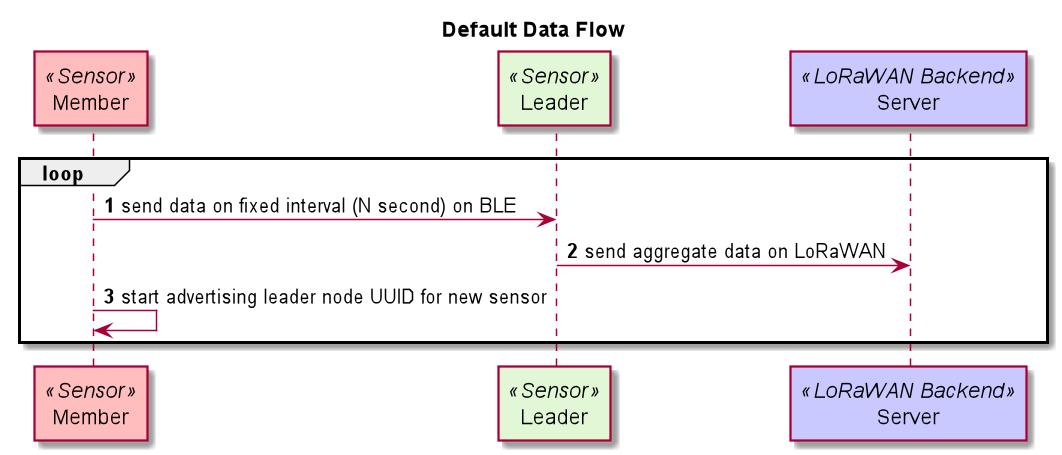
\includegraphics[width=13cm]{figures/グループ化の通信方式.png}
    \caption{グループ化の通信方式}
    \label{fig:default_data_flow}
    \end{center}
\end{figure}